% enable this to activate the version for PRINT
% disable this to make the pdf symmetric and without white pages
% => asymmetric alternating left/right margins
% \newcommand*{\printversion}{}%

%% | ---------------- document meta information --------------- |

\newcommand{\Author}{Adam El Ghaib}
\newcommand{\Department}{Department of Cybernetics}
\newcommand{\Supervisor}{Ing. Robert Pěnička, Ph.D.}
\newcommand{\SupervisorSpecialist}{Ing. Robert Pěnička, Ph.D.}
\newcommand{\Programme}{Cybernetics and Robotics (Space Master)}
\newcommand{\Field}{"""""""}
\newcommand{\Title}{Improving Sim-to-Real transfer of Learning-based Policies for Quadcopter Racing through Domain Randomization}
\newcommand{\Keywords}{Unmanned Aerial Vehicles, Automatic Control}
\newcommand{\KlicovaSlova}{Bezpilotní Prostředky, Automatické Řízení}
\newcommand{\Year}{2025}
\newcommand{\Month}{January}
\newcommand{\Date}{\Month~\Year}
\newcommand{\Location}{Prague}


%% | ---------------------- configuration --------------------- |

% most of the configuration stuff happens here
\input{src/document_setup.tex}

%% | ---------------------- the contents ---------------------- |

\begin{document}

% this will prevent unwanted line overflows
% http://latexref.xyz/_005cfussy-_0026-_005csloppy.html
\sloppy

\pagenumbering{roman}

%% --------------------------------------------------------------
%% |                         Title page                         |
%% --------------------------------------------------------------

\input{src/title}

% set up the page style for the "intro" pages
\pagestyle{plain}

%% --------------------------------------------------------------
%% |                       Acknowledgments                      |
%% --------------------------------------------------------------

\conditionalClearPage

% %!TEX root = ../main.tex

\section*{Acknowledgments}

I would like to express my gratitude to my supervisor, Ing. Robert Pěnička, Ph.D for his guidance and valuable advice throughout this thesis.
Also to the entire MRS group at CTU, particularly to the agile flight department, for the enjoyable environemnt and all the insightful discussions.
Finally, I would like to thank my family and friends for their unconditional support.

\vspace{2.5cm}


%% --------------------------------------------------------------
%% |                         Assignment                         |
%% --------------------------------------------------------------

\conditionalClearPage

% 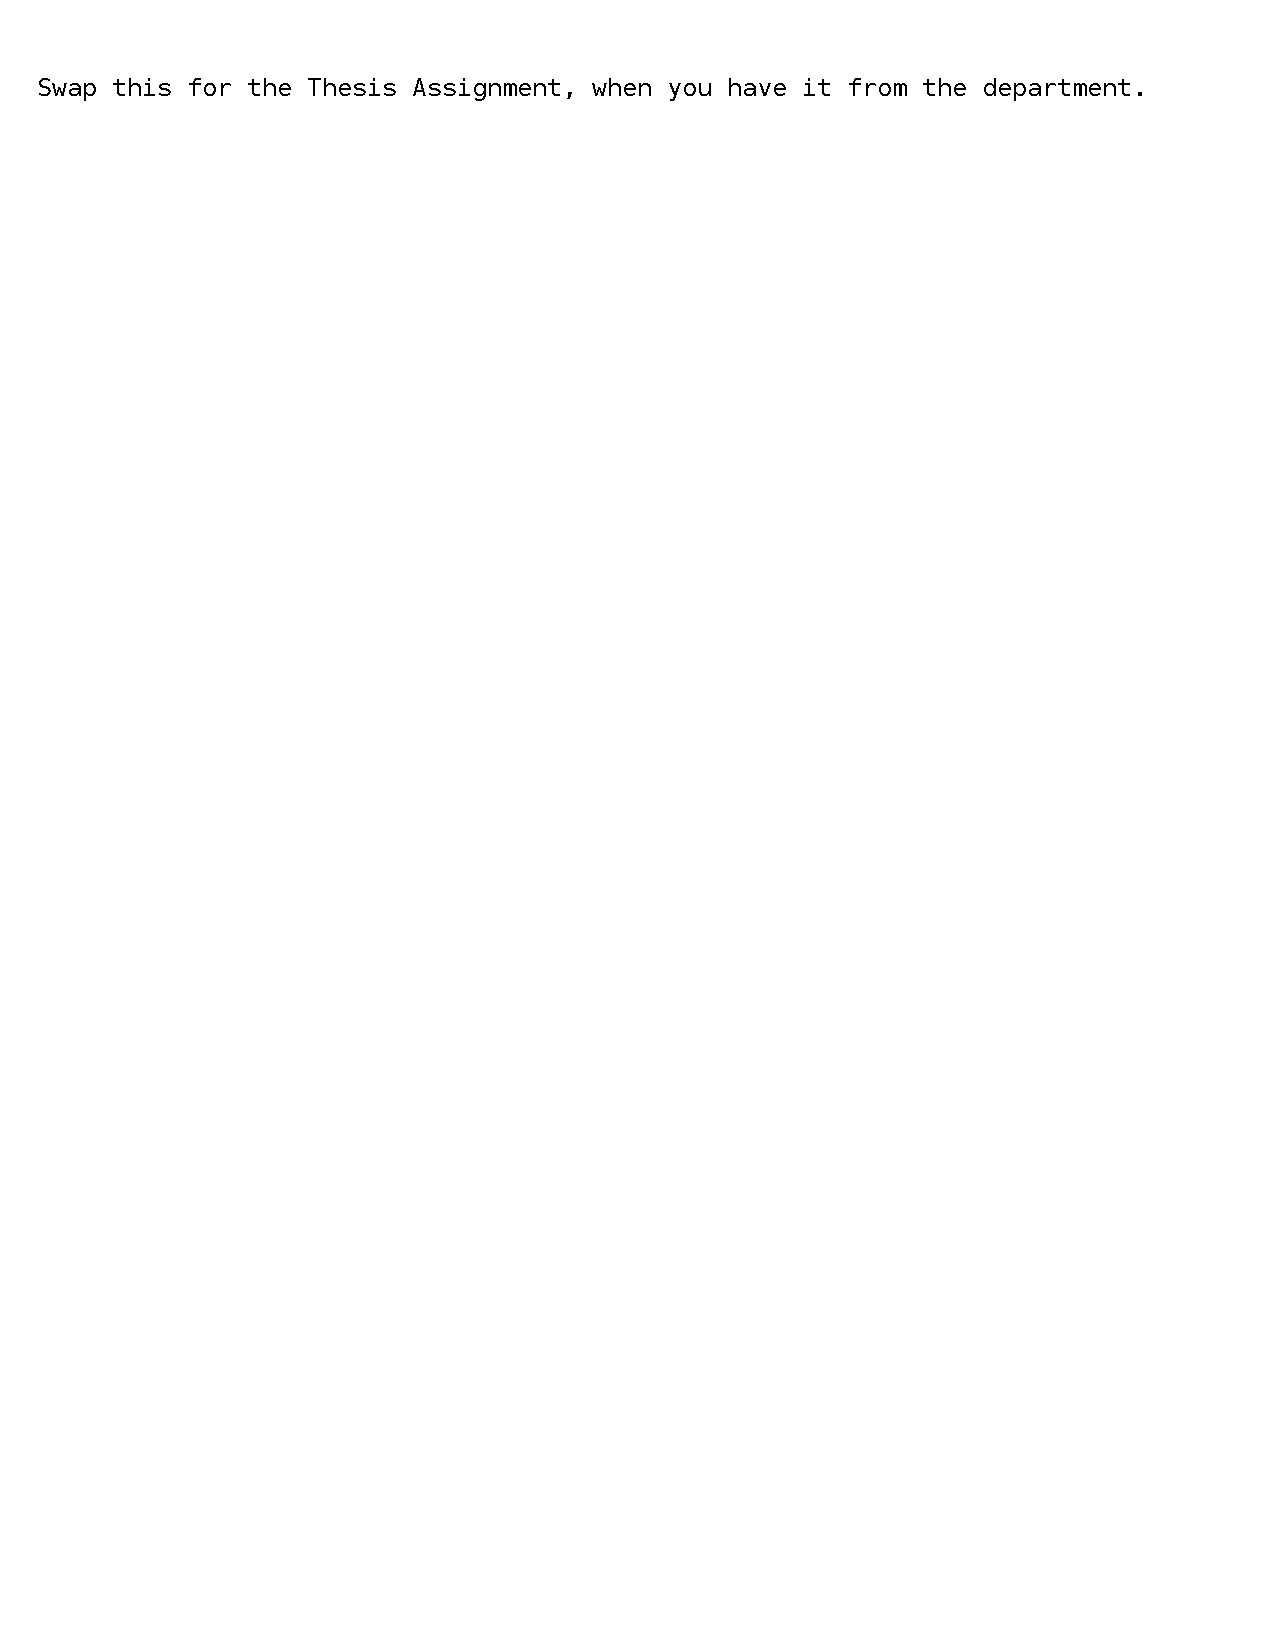
\includepdf{src/assignment.pdf}

%% --------------------------------------------------------------
%% |                         Declaration                        |
%% --------------------------------------------------------------

\conditionalClearPage

% \input{src/declaration.tex}

%% --------------------------------------------------------------
%% |                          Abstracts                         |
%% --------------------------------------------------------------

\conditionalClearPage

%!TEX root = ../main.tex

\begin{changemargin}{0.8cm}{0.8cm}

~\vfill{}

\section*{Abstract}
\vskip 0.5em

In \ac{ADR}, quadrotors operate near their physical limits to minimize lap times while navigating a sequence of gates.
This requires an efficient pipeline combining localization, planning and control.
\ac{RL} offers a promising solution, yet policies often fail to transfer from the simulated environments to real world scenarios, known as the \ac{s2r} gap.
This work addresses this issue by applying \ac{DR} to \ac{ADR} control policies.
Four policies were trained in a custom simulator and evaluated in Gazebo with three  randomized drones at levels of (10\%, 20\%, 30\%).
Performance was measured using success rate and lap time. Results show that moderate randomization (10–20\%) provides the best balance between robustness and speed, improving transferability without degrading performance.


\vskip 1em

{\bf Keywords} \Keywords

\vskip 2.5cm

\end{changemargin}


\conditionalClearPage

% %!TEX root = ../main.tex

\begin{changemargin}{0.8cm}{0.8cm}

~\vfill{}

\section*{Abstrakt}
\vskip 0.5em

\todo{Check with someone czech :3}

Model-free \ac{RL} výrazně zlepšilo výkon autonomního závodění dronů, avšak stále trpí nízkou efektivitou využití vzorků.
Geometrické řízení poskytuje plynulost a agresivitu požadovanou při závodění, je však omezeno nutností ručního ladění regulačních zesílení.
Tato diplomová práce zkoumá, zda může přímé \ac{BPTT} zvýšit efektivitu využití vzorků oproti standardnímu algoritmu \ac{PPO} při zachování srovnatelného výkonu a zda se naučená adaptivní zesílení mohou ukázat jako účinnější než pevně nastavená zesílení v geometrickém řízení.
V prostředí PyTorch jsme vytvořili diferencovatelný simulátor kvadrokoptéry a porovnali různé trénovací úlohy i abstrakce řízení.
Zjistili jsme, že \ac{BPTT} je ve scénáři s jedinou bránou až $\mathbf{5\times}$ efektivnější z hlediska využití vzorků, avšak vykazuje chamtivé chování a na kompletních závodních tratích nepřekonává algoritmus \ac{PPO}.
Ani adaptivní zesílení v námi navržené formulaci nepřinesla lepší výsledky než zesílení pevně nastavená.
Přesto řadič s pevnými zesíleními optimalizovaný pomocí \ac{PPO} dosahuje výkonu srovnatelného se současným stavem poznání (state of the art), čímž náš simulátor představuje vhodný základ pro další výzkum.

\vskip 1em

{\bf Klíčová slova} \KlicovaSlova

\vskip 2.5cm

\end{changemargin}


%% --------------------------------------------------------------
%% |                        Abbreviations                       |
%% --------------------------------------------------------------

\conditionalClearPage

\begin{changemargin}{0.8cm}{0.8cm}

~\vfill{}

\section*{Abbreviations}

% this will print only the used abbreviations
%!TEX root = ../main.tex

\begin{acronym}
  \acro{AC}[AC]{Actor Critic}
  \acro{ADE}[ADE]{Automatic Differentiation Engines}
  \acro{ADR}[ADR]{Autonomous Drone Racing}
  \acro{API}[API]{Application Programming Interface}
  \acro{BPTT}[BPTT]{Backpropagation Through Time}
  \acro{CNN}[CNN]{Convolutional Neural Network}
  % \acro{CNNs}[CNNs]{Convolutional Neural Networks}
  \acro{CRNN}[CRNN]{Convolutional Recurrent Neural Network}
  \acro{CTBR}[CTBR]{Collective Thrust and Body Rates}
  \acro{CTU}[CTU]{Czech Technical University}
  \acro{DC}{Direct Current}
  \acro{DFBC}[DFBC]{Differential Flatness Based Control}
  \acro{DP}{Dynamic Programming}
  \acro{DQN}{Deep Q-Learning}
  % \acro{DOF}[DOF]{degree-of-freedom}
  % \acro{DOFs}[DOFs]{Degrees-Of-Freedom}
  \acro{DR}[DR]{Domain Randomization}
  \acro{dof}[DoF]{Degrees of Freedom}
  \acro{EKF}[EKF]{Extended Kalman Filter}
  \acro{ESC}{Electronic Speed Controller}
  \acro{FOV}[FOV]{Field of View}
  \acro{GD}[GD]{Gradient Descent}
  \acro{GNSS}[GNSS]{Global Navigation Satellite System}
  \acro{GPS}[GPS]{Global Positioning System}
  \acro{IMU}[IMU]{Inertial Measurement Unit}
  \acro{LiDAR}[LiDAR]{Light Detection and Ranging}
  \acro{LiPo}[LiPo]{Lithium Polymer}
  \acro{LKF}[LKF]{Linear Kalman Filter}
  \acro{LTI}[LTI]{Linear time-invariant}
  \acro{MAV}[MAV]{Micro Aerial Vehicle}
  \acro{MDP}[MDP]{Markov Decision Process}
  \acro{MSE}[MSE]{Mean Square Error}
  \acro{ML}[ML]{Machine Learning}
  \acro{MLP}[MLP]{Multi-Layer Perceptron}
  % \acro{MLPs}[MLPs]{Multi-Layer Perceptrons}
  \acro{MPC}[MPC]{Model Predictive Control}
  \acro{MRS}[MRS]{Multi-robot Systems Group}
  \acro{NN}{Neural Network}
  \acro{OCP}[OCP]{Optimal Control Problem}
  % \acro{OCPs}[OCPs]{Optimal Control Problems}
  \acro{PID}{Proportional Integral Derivative}
  \acro{PMP}[PMP]{Pontryagin's Maximum Principle}
  \acro{POMDP}[POMDP]{Partially Observable Markov Decision Process}
  \acro{PPO}[PPO]{Proximal Policy Optimization}
  \acro{QP}[QP]{Quadratic Programming}
  \acro{RL}[RL]{Reinforcement Learning}
  \acro{RSSM}[RSSM]{Recurrent State Space Model}
  \acro{RMSP}[RMSProp]{Root Mean Square Propagation}
  \acro{RMSE}{Root Mean Square Error}
  \acro{ROS}[ROS]{Robot Operating System}
  \acro{RTK}[RTK]{Real-time Kinematics}
  \acro{SLAM}[SLAM]{Simultaneous Localization And Mapping}
  \acro{SR}{Success Rate}
  \acro{SRT}[SRT]{Single Rotor Thrust}
  \acro{s2r}[S2R]{Simulation-to-Reality}
  \acro{S2S}[S2S]{Simulation-to-Simulation}
  \acro{LVHR}[LVHR]{Linear Velocities and Heading Rate}
  \acro{TRPO}[TRPO]{Trust Region Policy Optimization}
  \acro{TWR}[TWR]{Thrust to Weight Ratio}
  \acro{UAV}[UAV]{Unmanned Aerial Vehicle}
  \acro{UGV}[UGV]{Unmanned Ground Vehicle}
  \acro{UKF}[UKF]{Unscented Kalman Filter}
  \acro{VIO}[VIO]{Visual Inertial Odometry}

\end{acronym}


\vskip 2.5cm

\end{changemargin}

\conditionalClearPage

%% --------------------------------------------------------------
%% |                      Table of contents                     |
%% --------------------------------------------------------------

\tableofcontents

\conditionalClearPage

% set up the full page style with normal page numbering
\pagestyle{full}
\pagenumbering{arabic}

%% --------------------------------------------------------------
%% |                        Introduction                        |
%% --------------------------------------------------------------

%!TEX root = ../main.tex

\chapter{Introduction\label{chap:introduction}}

% First, introduce the reader to the research topic.
% Start with the most general view and slowly converge to the particular field, sub-field, and the challenges you face.
% You can cite others' work here \cite{baca2021mrs}.

In the context of drone racing, where quadcopters are pushed to their physical and computational limits, there is a growing trend toward using neural networks for control.
As demonstrated in \cite{baca2021mrs}, this approach has made it possible to outperform some of the world's most skilled human pilots.

These neural networks controllers are tipically trained using \ac{RL} algorithms.
Due to the sample ineffiency of \ac{RL} and the high cost of collecting real-world flight data, training is performed in simulated environments that provide a safe and scalable alternative.
Despite this, the resulting control policies often perform worse than expected or fail to transfer to real-world scenarios altogether.
This discrepancy in the policy's performance between simulation and reality is known as the sim-to-real gap, and it mainly arises from an undesired overfit of the learned policy to the simulated environment.

% To mitigate this issue, improving the system's identification, using digital twins, or randomizing the domain, among other strategies, have shown to significantly reduce the sim-to-real gap.

% In this semesteral project, the focus has been placed on understanding and implementing \ac{DR} in learning-based control policies for quadcopter racing competitions.
% Key parameters from the drone's dynamics, perception, and observation spaces have been identified and randomized under different \ac{DR} configurations.
% Finally, {\color{red}{X}} randomized policies are analyzed and compared to non-randomized ones. Their performance is evaluated to assess how DR improves adaptability and transferability to real-world scenarios.

\section{Related works}

This section should contain related state-of-the-art works and their relation to the author's work.
We usually cite the original works like this \cite{benallegue2008high}.
You can also cite multiple papers at once like this \cite{baca2016embedded, baca2021mrs}.

Demonstrating that Domain Randomization (DR) can significantly increase the adaptability and robustness of autonomous systems, the work of Ferede et al. \cite{ferede2025} serves as the direct inspiration for this project. 
Their research showed that a DR-trained neural network controller could successfully generalize across various quadcopter platforms.
\section{Contributions}

(Note: rather than contribute this work aims to reproduce the results from \cite{ferede2025})

\section{Mathematical notation}

It is a good practice to define basic mathematical notation in the introduction.
See \reftab{tab:mathematical_notation} for an example.

\begin{table*}[!h]
  \scriptsize
  \centering
  \noindent\rule{\textwidth}{0.5pt}
  \begin{tabular}{lll}
    $\mathbf{x}$, $\bm{\alpha}$ & vector, pseudo-vector, or tuple\\
    $\mathbf{\hat{x}}$, $\bm{\hat{\omega}}$& unit vector or unit pseudo-vector\\
    $\mathbf{\hat{e}}_1, \mathbf{\hat{e}}_2, \mathbf{\hat{e}}_3$ & elements of the \emph{standard basis} \\
    $\mathbf{X}, \bm{\Omega}$ & matrix \\
    $\mathbf{I}$ & identity matrix \\
    $x = \mathbf{a}^\intercal\mathbf{b}$ & inner product of $\mathbf{a}$, $\mathbf{b}$ $\in \mathbb{R}^3$\\
    $\mathbf{x} = \mathbf{a}\times\mathbf{b}$ & cross product of $\mathbf{a}$, $\mathbf{b}$ $\in \mathbb{R}^3$\\
    $\mathbf{x} = \mathbf{a}\circ\mathbf{b}$ & element-wise product of $\mathbf{a}$, $\mathbf{b}$ $\in \mathbb{R}^3$ \\
    $\mathbf{x}_{(n)}$ = $\mathbf{x}^\intercal\mathbf{\hat{e}}_n$ & $\mathrm{n}^{\mathrm{th}}$ vector element (row), $\mathbf{x}, \mathbf{e} \in \mathbb{R}^3$\\
    $\mathbf{X}_{(a,b)}$ & matrix element, (row, column)\\
    $x_{d}$ & $x_d$ is \emph{desired}, a reference\\
    $\dot{x}, \ddot{x}, \dot{\ddot{x}}$, $\ddot{\ddot{x}}$ & ${1^{\mathrm{st}}}$, ${2^{\mathrm{nd}}}$, ${3^{\mathrm{rd}}}$, and ${4^{\mathrm{th}}}$ time derivative of $x$\\
    $x_{[n]}$ & $x$ at the sample $n$ \\
    $\mathbf{A}, \mathbf{B}, \mathbf{x}$ & LTI system matrix, input matrix and input vector\\
    \emph{SO(3)} & 3D special orthogonal group of rotations\\
    \emph{SE(3)} & \emph{SO(3)}~$\times~\mathbb{R}^3$, special Euclidean group\\
  \end{tabular}
  \noindent\rule{\textwidth}{0.5pt}
  \caption{Mathematical notation, nomenclature and notable symbols.}
  \label{tab:mathematical_notation}
\end{table*}


%% --------------------------------------------------------------
%% |                        Methodology                         |
%% --------------------------------------------------------------

%!TEX root = ../main.tex

\chapter{Methodology\label{chap:how_to}}

\section{Problem definition}
We will define a domain as a subset of all the possible \ac{MDP} environments.
A standard domain is characterized by a 4-tuple $\mathcal{D} = (S, A, P, R)$ where:

\begin{itemize}
    \item $\mathbf{S:}$ denotes a set of states called the state space.
    \item $\mathbf{A:}$ is the set of actions called the action space.
    \item $\mathbf{P(s'|s, a):}$ is the probability that a given action $a \subset A$, at state $s \subset S$ will lead to a new state $s' \subset S$. 
    \item $\mathbf{R(s',s,a):}$ is the inmediate reward, or expected inmediate reward, recived for transitioning from $s$ to $s'$ after performing action $a$. 
\end{itemize}
From the source domain, $\mathcal{D}_s$, (i.e. simulation), we can control a set of N parameters of the variable aspects of each environment that define a configuration vector, $\vec{\xi} = [\xi_1, \xi_2, ..., \xi_N]$.
Examples of $\xi$ can include:

\begin{tabular}{c|c}

    Physical properties & $\xi_{\text{mass}}, \ \xi_{\text{inertia}}, \ \xi_{\text{drag}}, \ \xi_{\text{gravity}}$ \\
    Perception properties & $\xi_{\text{sensor\_noise}}, \ \xi_{\text{sensor\_latency}}$ \\
    Viual properties & $\xi_{\text{lighting}}, \ \xi_{\text{texture}}, \ \xi_{\text{fov}}$ \\
    Scene properties & $\xi_{\text{gate\_pos}}, \ \xi_{\text{gate\_size}}, , \ \xi_{\text{gate\_num}}$ \\
    
\end{tabular}

Each configuration is sampled from a randomization space, $\vec{\xi} \in \Xi \subset \Re^N$, with a probability distribution $\vec{\xi} \sim p(\vec{\xi})$.
Where the parameters are bounded to be within an interval $\xi_i \in [\xi_i^{\text{low}}, \xi_i^{\text{high}}]$ \cite{weng2019DR}. 

At the start of every training episode, a new environment insance is created by sampling a new configuration vector $\vec{\xi}$ from the distribution $p(\vec{\xi})$. 
Therefore, the agent will interact with a specific \ac{MDP} environment, that is to say, a specific domain $\mathcal{D}_{\vec{\xi}}$. 
This way, the agent can collect data from a vareity of environments that otherwise would reamain unexplored. 
\begin{figure}[H]
  \centering

  \begin{adjustbox}{max totalsize={0.5\textwidth}{0.4\textheight}, center}
    

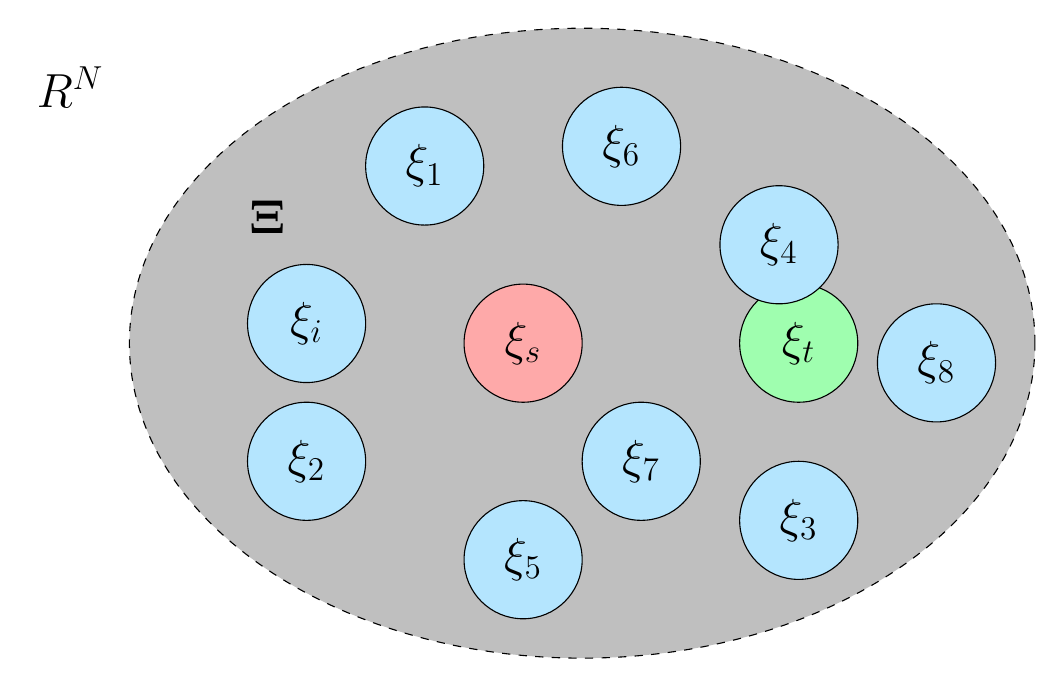
\begin{tikzpicture}[node distance=1cm, auto,]
\tikzstyle{every node}=[font=\LARGE]
\draw [ fill=gray!50, dashed] (8.25,7.75) ellipse (5.75cm and 4cm);
% \draw [dashed] (9.25 ,7.75) ellipse (3.25cm and 2cm);
\draw [ dashed] (14,11.75) ellipse (0cm and 0cm);
\draw [ dashed] (13,11.5) ellipse (0cm and 0cm);
\draw [ fill={rgb,255:red,180; green,229; blue,254} ] (4.75,8) circle (0.75cm) node {\LARGE $\xi_i$};
\draw [ fill={rgb,255:red,159; green,254; blue,175} ] (11,7.75) circle (0.75cm) node {\LARGE $\xi_t$};
\draw [ fill={rgb,255:red,180; green,229; blue,254} ] (6.25,10) circle (0.75cm) node {\LARGE $\xi_1$};
\draw [ fill={rgb,255:red,180; green,229; blue,254} ] (4.75,6.25) circle (0.75cm) node {\LARGE $\xi_2$};
% \draw [ fill={rgb,255:red,180; green,229; blue,254} ] (9.25,9) circle (0cm) node {\LARGE $\xi_3$};
% \draw [ fill={rgb,255:red,180; green,229; blue,254} ] (10,9) circle (0cm) node {\LARGE $\xi_4$};
\draw [ fill={rgb,255:red,180; green,229; blue,254} ] (11,5.5) circle (0.75cm) node {\LARGE $\xi_3$};
\draw [ fill={rgb,255:red,180; green,229; blue,254} ] (10.75,9) circle (0.75cm) node {\LARGE $\xi_4$};
\draw [ fill={rgb,255:red,180; green,229; blue,254} ] (7.5,5) circle (0.75cm) node {\LARGE $\xi_5$};
\draw [ fill={rgb,255:red,180; green,229; blue,254} ] (8.75,10.25) circle (0.75cm) node {\LARGE $\xi_6$};
\draw [ fill={rgb,255:red,180; green,229; blue,254} ] (9,6.25) circle (0.75cm) node {\LARGE $\xi_7$};
\draw [ fill={rgb,255:red,180; green,229; blue,254} ] (12.75,7.5) circle (0.75cm) node {\LARGE $\xi_8$};
\draw [ fill={rgb,255:red,254; green,169; blue,169} ] (7.5,7.75) circle (0.75cm) node {\LARGE $\xi_s$};
\node [font=\LARGE] at (4.25, 9.35) {$\mathbf{\Xi}$};
% \node [font=\LARGE] at (7.75, 9.25) {$\mathbf{\Theta}$};
\node [font=\LARGE] at (1.75, 11) {$\mathbb{R^N}$};


    
\end{tikzpicture}

  \end{adjustbox}

  \caption{Red and green the source and target domains respectively. In blue, differents instances of the randomized source space (all represented domains with the same size, $N$). }
  \label{fig:pgfplots_diagram}
\end{figure}
Hereby, during training, the neural network weights and biases $\theta$ are optimized to maximize the expected reward $R$ across a distribution of randomized domains.
With th objective of finding the optimal, $\theta^*$.
\begin{equation}
    \theta ^* = \arg \max_{\theta} \mathbb{E}_{\vec{\xi}\sim\Xi} \left[\mathbb{E}_{\pi_\theta,\tau\sim D_\xi}[R(\tau)] \right]
\end{equation}


And it will be able to react to certain unseen variations of the randomization space.
More specifically, from the 

% Hereby, the policy will be exposed to a rich varaeity of environments 
% Examples of randomization parameters could include physical properties such as $\xi_\text{mass},\ \xi_\text{inertia},\ \xi_\text{drag}$
\section{Quadcopter model}


\section{\ac{RL} set-up}



\begin{figure}[h]
  \centering

  \begin{adjustbox}{max totalsize={0.5\textwidth}{1.0\textheight}, center}
    \tikzset{
  >=latex, % for default LaTeX arrow head
  node/.style={thick,circle,draw=myblue,minimum size=22,inner sep=0.5,outer sep=0.6},
  node in/.style={node,green!20!black,draw=mygreen!30!black,fill=mygreen!25},
  node hidden/.style={node,blue!20!black,draw=myblue!30!black,fill=myblue!20},
  node convol/.style={node,orange!20!black,draw=myorange!30!black,fill=myorange!20},
  node out/.style={node,red!20!black,draw=myred!30!black,fill=myred!20},
  connect/.style={thick,mydarkblue}, %,line cap=round
  connect arrow/.style={-{Latex[length=4,width=3.5]},thick,mydarkblue,shorten <=0.5,shorten >=1},
  node 1/.style={node in}, % node styles, numbered for easy mapping with \nstyle
  node 2/.style={node hidden},
  node 3/.style={node out}
}
\def\nstyle{int(\lay<\Nnodlen?min(2,\lay):3)} % map layer number onto 1, 2, or 3

\begin{tikzpicture}[x=2.2cm,y=1.4cm]
  \message{^^JNeural network, shifted}
  \readlist\Nnod{4,5,5,5,3} % array of number of nodes per layer
  \readlist\Nstr{n,m,m,m,k} % array of string number of nodes per layer
  \readlist\Cstr{\strut x,a^{(\prev)},a^{(\prev)},a^{(\prev)},y} % array of coefficient symbol per layer
  \def\yshift{0.5} % shift last node for dots
  
  \message{^^J  Layer}
  \foreachitem \N \in \Nnod{ % loop over layers
    \def\lay{\Ncnt} % alias of index of current layer
    \pgfmathsetmacro\prev{int(\Ncnt-1)} % number of previous layer
    \message{\lay,}
    \foreach \i [evaluate={\c=int(\i==\N); \y=\N/2-\i-\c*\yshift;
                 \index=(\i<\N?int(\i):"\Nstr[\lay]");
                 \x=\lay; \n=\nstyle;}] in {1,...,\N}{ % loop over nodes
      % NODES
      \node[node \n] (N\lay-\i) at (\x,\y) {$\Cstr[\lay]_{\index}$};
      
      % CONNECTIONS
      \ifnum\lay>1 % connect to previous layer
        \foreach \j in {1,...,\Nnod[\prev]}{ % loop over nodes in previous layer
          \draw[connect,white,line width=1.2] (N\prev-\j) -- (N\lay-\i);
          \draw[connect] (N\prev-\j) -- (N\lay-\i);
          %\draw[connect] (N\prev-\j.0) -- (N\lay-\i.180); % connect to left
        }
      \fi % else: nothing to connect first layer
      
    }
    \path (N\lay-\N) --++ (0,1+\yshift) node[midway,scale=1.5] {$\vdots$};
  }
  
  % LABELS
  \node[above=1,align=center,mygreen!60!black] at (N1-2.90) {input\\[-0.2em]layer};
  \node[above=1,align=center,myblue!60!black] at (N3-2.90) {hidden layers};
  \node[above=1,align=center,myred!60!black] at (N\Nnodlen-2.90) {output\\[-0.2em]layer};
  
\end{tikzpicture}
  \end{adjustbox}

  \caption{Red and green the source and target domains respectively. In blue, differents instances of the randomized source space (all represented domains with the same size, $N$). }
  \label{fig:nn}
\end{figure}

\section{\ac{DR} configurations}



%% --------------------------------------------------------------
%% |                          Results                           |
%% --------------------------------------------------------------

%!TEX root = ../main.tex

\chapter{Results\label{chap:results}}

Summarize the achieved results.
Can be similar as an abstract or an introduction, however, it should be written in past tense.


%% --------------------------------------------------------------
%% |                         Conclusion                         |
%% --------------------------------------------------------------

%!TEX root = ../main.tex

\chapter{Conclusion \label{chap:conclusion}}

In this thesis, we developed a differentiable simulator envirionment to efficently train neural control policies for autonomous drone racing.
The simulator leverages automatic differentiation to backpropagate the gradients from a loss function to the network parameters, increasing the sample efficeny over \textbf{7x} compared to proximal policy optimization, a standard model-free reinforcement learning algorithm.
It includes domain randomization to prevent the policy from overfitting and to improve transferability to the real-world environment.
It supports four control abstractions, going from direct motor comands to a geometric controller with adaptive gains. 
% and evaluated their sample efficency, tracking performance and robustness agains external disturbances.
Since the motor model degreades the gradient quality, we implement a surrogate gradient for the backporopagation, in \autoref{sec:sur_grad} we show that this improves the optimization process.

In \autoref{subsec:sample_eff}, we find that the velocity controllers working on the special orthogonal group ${SO}(3)$ converge 3 times faster than the \ac{CTBR} controller and 6 times faster than the \ac{SRT} controller.
Training is implemented in a curriculum fashion, in which we increase the speed of the trajecotry when the tracking error is lower than a certain threshold.
With this approach, and the loss function proposed in \autoref{subsec::TT} we achieve a suboptimal tracking up to $10~\mathrm{m/s}$ corrpesonding to only $60\%$ of the optimal racing trajectory.
The control abstraction that obtains the best tracking error is the \ac{LVHR}, the agumented version of this controller, which outputs the gains of the inner geometric controller has similar tracking results.
However, in \autoref{subsec:robust} , the \ac{LVHR} controller showed to be the less robust to external disturbances, while its augmented verison seemd to compensate well to external distubances.
Nonetheless, with the obtained results we conclude that \ac{CTBR} controller achieves the best balance in terms of sample efficency, performance and robsutness.

Aditionally, during the MRS test campaing in on the 16th of April 2026, we deployed the \ac{CTBR} controller on a real UAV platfrom. 
At this time, the simulator did not model motor delay, aerodynamic effects or noise in state estimation, which lead to a poor tracking performance wit an \ac{RMSE} of $6.11~\mathrm{m}$. 
However, the controller was still able to stably track the trajectory, which underscores the importance of using domain randomization.

Finally in \autoref{sec:baseline}, we compare our model-based reinforcement learning approach using \ac{BPTT} to model-free reinforcement learning using \ac{PPO}.




%% --------------------------------------------------------------
%% |                         Example                      |
%% --------------------------------------------------------------

% \input{src/example.tex}

%% --------------------------------------------------------------
%% |                         References                         |
%% --------------------------------------------------------------

\chapter{References}

\printbibliography[heading=none,title={}]

%% --------------------------------------------------------------
%% |                         Appendices                         |
%% --------------------------------------------------------------

\appendix
\renewcommand\chaptername{Appendix}

\renewcommand{\thechapter}{A}
\renewcommand\chaptername{Appendix A}


\chapter{Appendix A}

\section{Simulator Validation}\label{sec:qualitative}
As detailed in \autoref{sec:sim_frame}, our simulator utilizes a simplified model of quadrotor dynamics and aerodynamics. 
To maintain a computationally efficient and generalizable framework, we omit secondary effects such as battery depletion on thrust, complex aerodynamic effects, and the propellers rotational inertia. 
While these unmodeled dynamics can cumulatively lead to a significant sim-to-real gap, we aim to address this mismatch through \ac{DR}.
To validate the reliability of this simplified approach, we benchmark our simulator's behavior against Gazebo, a high-fidelity physics engine widely adopted by the robotics community. 
Specifically, we utilize the UAV models provided by the MRS UAV System within the Gazebo environment as our ground-truth reference for comparison.

We separelty asses the respones of the body rates against a unit step, a variable amplitude and a variable frequency signals.
\begin{figure}[H]
  \centering
  
\includegraphics[width=1.0\textwidth]{./fig/plots/omega-xy-val/hypotheses.pdf}
  \caption{Pitch/Roll responses to unit step, variable amblitude and variable frequency signals.}
  \label{fig:wx-y-val}
\end{figure}
For the pitch and roll responses, the behavior observed in Gazebo and in our simulator is consistent.
Minor discrepancies can be observed in the response of integration of the unit-step error, together with a slight overshoot in the variable-frequency signal.
\begin{figure}[H]
  \centering
  
\includegraphics[width=1.0\textwidth]{./fig/plots/omega-z-val/hypotheses.pdf}
  \caption{Yaw response to unit step, variable amblitude and variable frequency signals.}
  \label{fig:wz-val}
\end{figure}

Similarly, the yaw reponse are close but there is some mismathc on the variable freuqency signal.
In our simulator we saturate the yaw rate to $\pm 3$ rad/s and the yaw acceleartion to $\pm 5$ rad/$s^2$ to match with Gazebo. 
\end{document}
